\section{PWM}
PWM eller pulsbredde modulation er en måde et firkant signal, hvor tiden signalet er højt kan justeres. Procentdelen hvor signalet er højt, bliver udregnet i forhold til én periode, hvilket er længden imellem 2 frekvenser. Duty cyclen på et PWM signal er mellem 0 og 100\%. F.eks. svarer 0\% til at der intet signal er og 50\% svare til at signalet er høj halvdelen af tiden. Dvs. et PWM signal med en duty cycle på 50\% og en amplityde på 10 V, vil således være et PWM signal på 5 V. Frekvensen på PWM signalet skal blot være tilstrækkelig høj, så belastningen ikke blive påvirket af det svingende signal. 
\\
\\
PWM kan genereres af modulet Output compare på microprocessoren. Da ADC blev konfigureret ved at sætte de enkelte registre, valgte gruppen at prøve at bruge plib eller peripheral library til at opsætte PWM som et alternativ til at opsætte de indivuduelle registre. Plib er et bibliotek som giver simpel tilgang til hardware funktioner uden at skulle skrive til specifikke registre\fxnote{kilde lige under}.
%http://microchip.wikidot.com/harmony:overview-plib

\begin{figure}[h!]
  \centering
  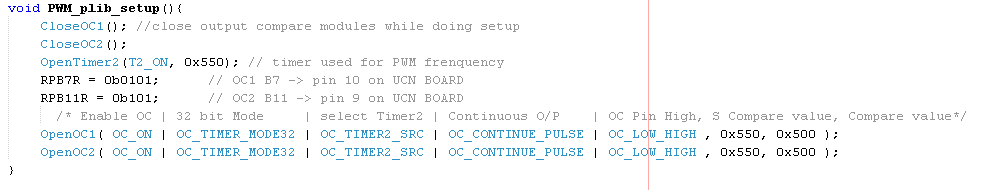
\includegraphics[width=1.0\textwidth]{figures/PWM_setup.png}
  \caption{PWM setup kode.}
  \label{PWM_setup}
\end{figure} 

PWM opsætning er skrevet med udgangspunkt i et eksempel fundet i "pic32-lib-help" fra microchip. \fxnote{evt. kilde til plib} 

På figur \ref{PWM_setup} ses opsæting af PWM ved brug af plib registreret. Det første der foretages er, at output compare modulet bliver slukket, således det senere kan åbnes med de valgte opsætninger. 

Her har gruppen valgt at bruge pin 9 og 10 på UCN bordet til PWM. Disse anvendes ved at skrive til output pin selection registreret (RPnR register) da disse ikke bliver sat i plib. \fxnote{kilde til side 132 pic32 family}

Af tidsmæssige årsager valgte gruppen at benytte plib, for også at få lidt erfaring med en anden implementerings metode. Dette er gjort frem for at sætte enkelte registre. Koden kan skrives nemmere, da opsætningsmulighederne er samlet et sted, og funktioner er allerede konstrueret. Dog mangler opsætningen af hvilken pin output der bruges, derfor kan registre ikke helt ungåes.

% hvad er PWM
% hvordan vi implementerede
% evt sammenligning?
